% Options for packages loaded elsewhere
\PassOptionsToPackage{unicode}{hyperref}
\PassOptionsToPackage{hyphens}{url}
\PassOptionsToPackage{dvipsnames,svgnames,x11names}{xcolor}
%
\documentclass[
  xelatex,
  ja=standard]{bxjsarticle}

\usepackage{amsmath,amssymb}
\usepackage{iftex}
\ifPDFTeX
  \usepackage[T1]{fontenc}
  \usepackage[utf8]{inputenc}
  \usepackage{textcomp} % provide euro and other symbols
\else % if luatex or xetex
  \usepackage{unicode-math}
  \defaultfontfeatures{Scale=MatchLowercase}
  \defaultfontfeatures[\rmfamily]{Ligatures=TeX,Scale=1}
\fi
\usepackage{lmodern}
\ifPDFTeX\else  
    % xetex/luatex font selection
  \setmainfont[BoldFont=Noto Sans CJK JP]{Noto Serif CJK JP}
\fi
% Use upquote if available, for straight quotes in verbatim environments
\IfFileExists{upquote.sty}{\usepackage{upquote}}{}
\IfFileExists{microtype.sty}{% use microtype if available
  \usepackage[]{microtype}
  \UseMicrotypeSet[protrusion]{basicmath} % disable protrusion for tt fonts
}{}
\makeatletter
\@ifundefined{KOMAClassName}{% if non-KOMA class
  \IfFileExists{parskip.sty}{%
    \usepackage{parskip}
  }{% else
    \setlength{\parindent}{0pt}
    \setlength{\parskip}{6pt plus 2pt minus 1pt}}
}{% if KOMA class
  \KOMAoptions{parskip=half}}
\makeatother
\usepackage{xcolor}
\setlength{\emergencystretch}{3em} % prevent overfull lines
\setcounter{secnumdepth}{5}
% Make \paragraph and \subparagraph free-standing
\ifx\paragraph\undefined\else
  \let\oldparagraph\paragraph
  \renewcommand{\paragraph}[1]{\oldparagraph{#1}\mbox{}}
\fi
\ifx\subparagraph\undefined\else
  \let\oldsubparagraph\subparagraph
  \renewcommand{\subparagraph}[1]{\oldsubparagraph{#1}\mbox{}}
\fi


\providecommand{\tightlist}{%
  \setlength{\itemsep}{0pt}\setlength{\parskip}{0pt}}\usepackage{longtable,booktabs,array}
\usepackage{calc} % for calculating minipage widths
% Correct order of tables after \paragraph or \subparagraph
\usepackage{etoolbox}
\makeatletter
\patchcmd\longtable{\par}{\if@noskipsec\mbox{}\fi\par}{}{}
\makeatother
% Allow footnotes in longtable head/foot
\IfFileExists{footnotehyper.sty}{\usepackage{footnotehyper}}{\usepackage{footnote}}
\makesavenoteenv{longtable}
\usepackage{graphicx}
\makeatletter
\def\maxwidth{\ifdim\Gin@nat@width>\linewidth\linewidth\else\Gin@nat@width\fi}
\def\maxheight{\ifdim\Gin@nat@height>\textheight\textheight\else\Gin@nat@height\fi}
\makeatother
% Scale images if necessary, so that they will not overflow the page
% margins by default, and it is still possible to overwrite the defaults
% using explicit options in \includegraphics[width, height, ...]{}
\setkeys{Gin}{width=\maxwidth,height=\maxheight,keepaspectratio}
% Set default figure placement to htbp
\makeatletter
\def\fps@figure{htbp}
\makeatother

\renewcommand{\thefootnote}{\arabic{footnote}}
\makeatletter
\@ifpackageloaded{tcolorbox}{}{\usepackage[skins,breakable]{tcolorbox}}
\@ifpackageloaded{fontawesome5}{}{\usepackage{fontawesome5}}
\definecolor{quarto-callout-color}{HTML}{909090}
\definecolor{quarto-callout-note-color}{HTML}{0758E5}
\definecolor{quarto-callout-important-color}{HTML}{CC1914}
\definecolor{quarto-callout-warning-color}{HTML}{EB9113}
\definecolor{quarto-callout-tip-color}{HTML}{00A047}
\definecolor{quarto-callout-caution-color}{HTML}{FC5300}
\definecolor{quarto-callout-color-frame}{HTML}{acacac}
\definecolor{quarto-callout-note-color-frame}{HTML}{4582ec}
\definecolor{quarto-callout-important-color-frame}{HTML}{d9534f}
\definecolor{quarto-callout-warning-color-frame}{HTML}{f0ad4e}
\definecolor{quarto-callout-tip-color-frame}{HTML}{02b875}
\definecolor{quarto-callout-caution-color-frame}{HTML}{fd7e14}
\makeatother
\makeatletter
\makeatother
\makeatletter
\makeatother
\makeatletter
\@ifpackageloaded{caption}{}{\usepackage{caption}}
\AtBeginDocument{%
\ifdefined\contentsname
  \renewcommand*\contentsname{目次}
\else
  \newcommand\contentsname{目次}
\fi
\ifdefined\listfigurename
  \renewcommand*\listfigurename{図一覧}
\else
  \newcommand\listfigurename{図一覧}
\fi
\ifdefined\listtablename
  \renewcommand*\listtablename{表一覧}
\else
  \newcommand\listtablename{表一覧}
\fi
\ifdefined\figurename
  \renewcommand*\figurename{図}
\else
  \newcommand\figurename{図}
\fi
\ifdefined\tablename
  \renewcommand*\tablename{表}
\else
  \newcommand\tablename{表}
\fi
}
\@ifpackageloaded{float}{}{\usepackage{float}}
\floatstyle{ruled}
\@ifundefined{c@chapter}{\newfloat{codelisting}{h}{lop}}{\newfloat{codelisting}{h}{lop}[chapter]}
\floatname{codelisting}{コード}
\newcommand*\listoflistings{\listof{codelisting}{コード一覧}}
\makeatother
\makeatletter
\@ifpackageloaded{caption}{}{\usepackage{caption}}
\@ifpackageloaded{subcaption}{}{\usepackage{subcaption}}
\makeatother
\makeatletter
\@ifpackageloaded{tcolorbox}{}{\usepackage[skins,breakable]{tcolorbox}}
\makeatother
\makeatletter
\@ifundefined{shadecolor}{\definecolor{shadecolor}{rgb}{.97, .97, .97}}
\makeatother
\makeatletter
\makeatother
\makeatletter
\makeatother
\ifLuaTeX
\usepackage[bidi=basic]{babel}
\else
\usepackage[bidi=default]{babel}
\fi
\babelprovide[main,import]{japanese}
% get rid of language-specific shorthands (see #6817):
\let\LanguageShortHands\languageshorthands
\def\languageshorthands#1{}
\ifLuaTeX
  \usepackage{selnolig}  % disable illegal ligatures
\fi
\usepackage[]{natbib}
\bibliographystyle{jecon}
\IfFileExists{bookmark.sty}{\usepackage{bookmark}}{\usepackage{hyperref}}
\IfFileExists{xurl.sty}{\usepackage{xurl}}{} % add URL line breaks if available
\urlstyle{same} % disable monospaced font for URLs
\hypersetup{
  pdftitle={平和の要因},
  pdfauthor={土井翔平},
  pdflang={ja},
  colorlinks=true,
  linkcolor={NavyBlue},
  filecolor={Maroon},
  citecolor={NavyBlue},
  urlcolor={NavyBlue},
  pdfcreator={LaTeX via pandoc}}

\title{平和の要因}
\usepackage{etoolbox}
\makeatletter
\providecommand{\subtitle}[1]{% add subtitle to \maketitle
  \apptocmd{\@title}{\par {\large #1 \par}}{}{}
}
\makeatother
\subtitle{国際公共政策学}
\author{土井翔平}
\date{2023-05-16}

\begin{document}
\maketitle
\ifdefined\Shaded\renewenvironment{Shaded}{\begin{tcolorbox}[frame hidden, interior hidden, breakable, borderline west={3pt}{0pt}{shadecolor}, sharp corners, enhanced, boxrule=0pt]}{\end{tcolorbox}}\fi

\hypertarget{ux306fux3058ux3081ux306b}{%
\section*{はじめに}\label{ux306fux3058ux3081ux306b}}
\addcontentsline{toc}{section}{はじめに}

軍事力(それに基づく抑止力)は万能の薬ではない。

\(\leadsto\)それ以外の戦争を回避する、平和を促進する要因の模索

\begin{enumerate}
\def\labelenumi{\arabic{enumi}.}
\tightlist
\item
  国際制度:国際的な武力行使の違法化とその違反に対する制裁、軍備の管理や縮小
\item
  民主主義:民主的な政治体制の国による戦争の回避
\item
  経済的相互依存:国家間の経済交流による平和の促進
\end{enumerate}

リベラルな平和、カント的平和\citep{oneal1997, oneal1999}\footnote{カントの「永遠平和のために」がこうした思想の潮流とする見方のため。}、リベラル国際秩序
(liberal international order: ILO)
\citep{ikenberry2009, ikenberry2018}などと呼ばれる。

\hypertarget{ux56fdux969bux5236ux5ea6ux3068ux5e73ux548c}{%
\section{国際制度と平和}\label{ux56fdux969bux5236ux5ea6ux3068ux5e73ux548c}}

多くの国内社会でそうであるように、ルール(制度)で暴力を止める。

\begin{itemize}
\tightlist
\item
  戦争(武力行使)の違法化
\item
  集団的安全保障
\item
  軍縮・不拡散
\end{itemize}

\hypertarget{ux6226ux4e89ux306eux9055ux6cd5ux5316}{%
\subsection{戦争の違法化}\label{ux6226ux4e89ux306eux9055ux6cd5ux5316}}

\hypertarget{ux6226ux9593ux671f}{%
\subsubsection{戦間期}\label{ux6226ux9593ux671f}}

第1次世界大戦\(\leadsto\)軍備拡大や同盟による平和の維持には限界

\(\leadsto\)戦争を行う権利を制限するルール (\textbf{jus ad bellum})
によって平和を維持しようとする動き\citep[第3章]{yamakage2012}

ウッドロー・ウィルソン米大統領の提案により\textbf{国際連盟} (the League
of Nations) が設立

\(\leadsto\)\href{https://avalon.law.yale.edu/20th_century/leagcov.asp}{国際連盟規約}:加盟国への戦争は加盟国全体の問題である。

\begin{tcolorbox}[enhanced jigsaw, rightrule=.15mm, breakable, bottomrule=.15mm, colback=white, left=2mm, toptitle=1mm, title=\textcolor{quarto-callout-note-color}{\faInfo}\hspace{0.5em}{\href{https://avalon.law.yale.edu/20th_century/leagcov.asp}{国際連盟規約} 第11条}, colbacktitle=quarto-callout-note-color!10!white, titlerule=0mm, coltitle=black, bottomtitle=1mm, arc=.35mm, opacitybacktitle=0.6, leftrule=.75mm, colframe=quarto-callout-note-color-frame, toprule=.15mm, opacityback=0]

Any war or threat of war, whether immediately affecting any of the
Members of the League or not, is hereby declared \textbf{a matter of
concern to the whole League}, and the League shall take any action that
may be deemed wise and effectual to safeguard the peace of nations. In
case any such emergency should arise the Secretary General shall on the
request of any Member of the League forthwith summon a meeting of the
Council.

\end{tcolorbox}

\begin{tcolorbox}[enhanced jigsaw, rightrule=.15mm, breakable, bottomrule=.15mm, colback=white, left=2mm, toptitle=1mm, title=\textcolor{quarto-callout-note-color}{\faInfo}\hspace{0.5em}{\href{https://avalon.law.yale.edu/20th_century/leagcov.asp}{国際連盟規約} 第16条}, colbacktitle=quarto-callout-note-color!10!white, titlerule=0mm, coltitle=black, bottomtitle=1mm, arc=.35mm, opacitybacktitle=0.6, leftrule=.75mm, colframe=quarto-callout-note-color-frame, toprule=.15mm, opacityback=0]

Should any Member of the League resort to war in disregard of its
covenants under Articles 12, 13 or 15, it shall ipso facto be deemed to
have committed \textbf{an act of war against all other Members of the
League}, which hereby undertake immediately to subject it to the
severance of all trade or financial relations, the prohibition of all
intercourse between their nationals and the nationals of the
covenant-breaking State, and the prevention of all financial, commercial
or personal intercourse between the nationals of the covenant-breaking
State and the nationals of any other State, whether a Member of the
League or not.

\end{tcolorbox}

\(\leadsto\)\href{https://avalon.law.yale.edu/20th_century/kbpact.asp}{\textbf{不戦条約}}(ケロッグ=ブリアン条約):戦争の放棄に各国が合意(1928年)

\begin{tcolorbox}[enhanced jigsaw, rightrule=.15mm, breakable, bottomrule=.15mm, colback=white, left=2mm, toptitle=1mm, title=\textcolor{quarto-callout-note-color}{\faInfo}\hspace{0.5em}{\href{https://avalon.law.yale.edu/20th_century/kbpact.asp}{不戦条約}第1条}, colbacktitle=quarto-callout-note-color!10!white, titlerule=0mm, coltitle=black, bottomtitle=1mm, arc=.35mm, opacitybacktitle=0.6, leftrule=.75mm, colframe=quarto-callout-note-color-frame, toprule=.15mm, opacityback=0]

The High Contracting Parties solemly declare in the names of their
respective peoples that they condemn recourse to war for the solution of
international controversies, and \textbf{renounce it, as an instrument
of national policy} in their relations with one another.

\end{tcolorbox}

\hypertarget{ux7b2c2ux6b21ux4e16ux754cux5927ux6226ux5f8c}{%
\subsubsection{第2次世界大戦後}\label{ux7b2c2ux6b21ux4e16ux754cux5927ux6226ux5f8c}}

国際連盟や不戦条約では第2次世界大戦を防止することはできず。

\(\leadsto\)戦後に設立された\textbf{国際連合} (the United
Nations):\textbf{武力行使禁止原則}が確立

\begin{tcolorbox}[enhanced jigsaw, rightrule=.15mm, breakable, bottomrule=.15mm, colback=white, left=2mm, toptitle=1mm, title=\textcolor{quarto-callout-note-color}{\faInfo}\hspace{0.5em}{\href{https://www.unic.or.jp/info/un/charter/text_japanese/}{国連憲章} 第2条3項}, colbacktitle=quarto-callout-note-color!10!white, titlerule=0mm, coltitle=black, bottomtitle=1mm, arc=.35mm, opacitybacktitle=0.6, leftrule=.75mm, colframe=quarto-callout-note-color-frame, toprule=.15mm, opacityback=0]

すべての加盟国は、その国際紛争を\textbf{平和的手段によって}国際の平和及び安全並びに正義を危くしないように\textbf{解決しなければならない}。

\end{tcolorbox}

\begin{tcolorbox}[enhanced jigsaw, rightrule=.15mm, breakable, bottomrule=.15mm, colback=white, left=2mm, toptitle=1mm, title=\textcolor{quarto-callout-note-color}{\faInfo}\hspace{0.5em}{\href{https://www.unic.or.jp/info/un/charter/text_japanese/}{国連憲章} 第2条4項}, colbacktitle=quarto-callout-note-color!10!white, titlerule=0mm, coltitle=black, bottomtitle=1mm, arc=.35mm, opacitybacktitle=0.6, leftrule=.75mm, colframe=quarto-callout-note-color-frame, toprule=.15mm, opacityback=0]

すべての加盟国は、その国際関係において、\textbf{武力による威嚇又は武力の行使を}、いかなる国の領土保全又は政治的独立に対するものも、また、国際連合の目的と両立しない他のいかなる方法によるものも\textbf{慎まなければならない}。

\end{tcolorbox}

\begin{itemize}
\tightlist
\item
  戦争を禁止した国際連盟規約とは異なり、武力による威嚇および武力行使
  (the threat or use of force) を禁止
\item
  武力行使禁止原則は慣習国際法(ニカラグア事件ICJ判決、1986年)
\end{itemize}

自衛権 (self-defense) の行使としての武力行使は例外として認められている。

\begin{tcolorbox}[enhanced jigsaw, rightrule=.15mm, breakable, bottomrule=.15mm, colback=white, left=2mm, toptitle=1mm, title=\textcolor{quarto-callout-note-color}{\faInfo}\hspace{0.5em}{\href{https://www.unic.or.jp/info/un/charter/text_japanese/}{国連憲章} 第51条}, colbacktitle=quarto-callout-note-color!10!white, titlerule=0mm, coltitle=black, bottomtitle=1mm, arc=.35mm, opacitybacktitle=0.6, leftrule=.75mm, colframe=quarto-callout-note-color-frame, toprule=.15mm, opacityback=0]

この憲章のいかなる規定も、国際連合加盟国に対して武力攻撃が発生した場合には、安全保障理事会が国際の平和及び安全の維持に必要な措置をとるまでの間、\textbf{個別的又は集団的自衛の固有の権利を害するものではない}。

\end{tcolorbox}

\begin{itemize}
\tightlist
\item
  国際法上、個別的自衛権と集団的自衛権の合法性は区別されていない。
\end{itemize}

\hypertarget{ux96c6ux56e3ux5b89ux5168ux4fddux969c}{%
\subsection{集団安全保障}\label{ux96c6ux56e3ux5b89ux5168ux4fddux969c}}

武力行使を国際法上、禁止したとしても、それだけでは意味はない。

\(\leadsto\)\textbf{集団的安全保障} (collective security)
\footnote{集団的自衛権とは似て非なるものなので、要注意。}の発明

\begin{itemize}
\tightlist
\item
  集団的安全保障:武力行使禁止原則に反した国に対して、他の全ての加盟国が制裁を加えることで、それを抑止する。
\end{itemize}

事実上、全ての加盟国で防衛同盟を結んでいることになる。

\begin{itemize}
\tightlist
\item
  同盟では敵が同盟の外部にいることが前提
\item
  集団安全保障では仮想敵が組織内部に存在することを前提
\end{itemize}

\begin{figure}

\begin{minipage}[t]{0.50\linewidth}

{\centering 

\raisebox{-\height}{

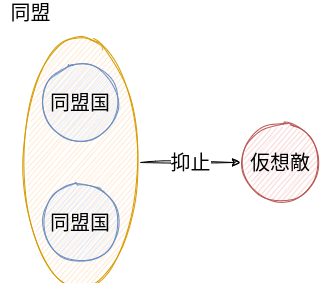
\includegraphics{figures/alliance.drawio.png}

}

\caption{同盟のイメージ}

}

\end{minipage}%
%
\begin{minipage}[t]{0.50\linewidth}

{\centering 

\raisebox{-\height}{

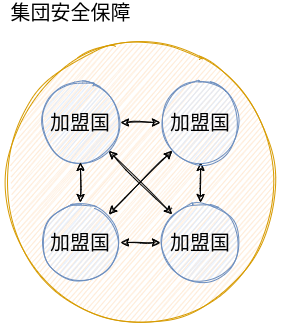
\includegraphics{figures/collective_security.drawio.png}

}

\caption{集団安全保障のイメージ}

}

\end{minipage}%

\end{figure}

\(\leadsto\)できる限り多くの国家が参加する\textbf{普遍的} (universal)
制度であるのが望ましい。

\begin{figure}[htpb]

{\centering \includegraphics{liberal_peace_files/mediabag/United_Nations_membe.PNG}

}

\caption{\href{https://commons.wikimedia.org/wiki/File:United_Nations_member_countries_world_map.PNG}{国連加盟国と加盟年}}

\end{figure}

\hypertarget{ux56fdux9023ux5b89ux5168ux4fddux969cux7406ux4e8bux4f1a}{%
\subsubsection{国連安全保障理事会}\label{ux56fdux9023ux5b89ux5168ux4fddux969cux7406ux4e8bux4f1a}}

\href{https://www.un.org/securitycouncil/}{\textbf{安全保障理事会}}
(Security Council: SC):国際連合において、集団安全保障を担う機関

\begin{figure}[htpb]

{\centering \includegraphics[width=0.5\textwidth,height=\textheight]{liberal_peace_files/mediabag/UN_security_council_.jpg}

}

\caption{\href{https://commons.wikimedia.org/wiki/File:UN_security_council_2005.jpg}{国連安全保障理事会}}

\end{figure}

\begin{tcolorbox}[enhanced jigsaw, rightrule=.15mm, breakable, bottomrule=.15mm, colback=white, left=2mm, toptitle=1mm, title=\textcolor{quarto-callout-note-color}{\faInfo}\hspace{0.5em}{\href{https://www.unic.or.jp/info/un/charter/text_japanese/}{国連憲章} 第24条1項}, colbacktitle=quarto-callout-note-color!10!white, titlerule=0mm, coltitle=black, bottomtitle=1mm, arc=.35mm, opacitybacktitle=0.6, leftrule=.75mm, colframe=quarto-callout-note-color-frame, toprule=.15mm, opacityback=0]

国際連合の迅速且つ有効な行動を確保するために、国際連合加盟国は、国際の平和及び安全の維持に関する\textbf{主要な責任}を安全保障理事会に負わせるものとし、且つ、安全保障理事会がこの責任に基く義務を果すに当って加盟国に代って行動することに同意する。

\end{tcolorbox}

\(\leadsto\)\textbf{平和に対する脅威}を認定し、必要な強制措置を決定

\begin{tcolorbox}[enhanced jigsaw, rightrule=.15mm, breakable, bottomrule=.15mm, colback=white, left=2mm, toptitle=1mm, title=\textcolor{quarto-callout-note-color}{\faInfo}\hspace{0.5em}{\href{https://www.unic.or.jp/info/un/charter/text_japanese/}{国連憲章} 第39条}, colbacktitle=quarto-callout-note-color!10!white, titlerule=0mm, coltitle=black, bottomtitle=1mm, arc=.35mm, opacitybacktitle=0.6, leftrule=.75mm, colframe=quarto-callout-note-color-frame, toprule=.15mm, opacityback=0]

安全保障理事会は、\textbf{平和に対する脅威}、平和の破壊又は侵略行為の存在を決定し、並びに、国際の平和及び安全を維持し又は回復するために、勧告をし、又は\textbf{第41条及び第42条に従っていかなる措置をとるかを決定する}。

\end{tcolorbox}

強制措置:非軍事(経済)制裁および軍事制裁

\begin{tcolorbox}[enhanced jigsaw, rightrule=.15mm, breakable, bottomrule=.15mm, colback=white, left=2mm, toptitle=1mm, title=\textcolor{quarto-callout-note-color}{\faInfo}\hspace{0.5em}{\href{https://www.unic.or.jp/info/un/charter/text_japanese/}{国連憲章} 第41条}, colbacktitle=quarto-callout-note-color!10!white, titlerule=0mm, coltitle=black, bottomtitle=1mm, arc=.35mm, opacitybacktitle=0.6, leftrule=.75mm, colframe=quarto-callout-note-color-frame, toprule=.15mm, opacityback=0]

安全保障理事会は、その決定を実施するために、\textbf{兵力の使用を伴わないいかなる措置}を使用すべきかを決定することができ、且つ、この措置を適用するように国際連合加盟国に要請することができる。\ldots{}

\end{tcolorbox}

\begin{tcolorbox}[enhanced jigsaw, rightrule=.15mm, breakable, bottomrule=.15mm, colback=white, left=2mm, toptitle=1mm, title=\textcolor{quarto-callout-note-color}{\faInfo}\hspace{0.5em}{\href{https://www.unic.or.jp/info/un/charter/text_japanese/}{国連憲章} 第42条}, colbacktitle=quarto-callout-note-color!10!white, titlerule=0mm, coltitle=black, bottomtitle=1mm, arc=.35mm, opacitybacktitle=0.6, leftrule=.75mm, colframe=quarto-callout-note-color-frame, toprule=.15mm, opacityback=0]

安全保障理事会は、第41条に定める措置では不充分であろうと認め、又は不充分なことが判明したと認めるときは、国際の平和及び安全の維持又は回復に必要な\textbf{空軍、海軍又は陸軍の行動}をとることができる。\ldots{}

\end{tcolorbox}

\begin{itemize}
\tightlist
\item
  脅威認定および強制措置の決定は国連憲章第7章に規定\(\leadsto\)これらが言及されている決議を7章決議
\end{itemize}

安全保障理事会は5つの\textbf{常任理事国} (permanent seat: \textbf{P5})
と10 (6) ヶ国の非常任理事国

\begin{tcolorbox}[enhanced jigsaw, rightrule=.15mm, breakable, bottomrule=.15mm, colback=white, left=2mm, toptitle=1mm, title=\textcolor{quarto-callout-note-color}{\faInfo}\hspace{0.5em}{\href{https://www.unic.or.jp/info/un/charter/text_japanese/}{国連憲章} 第23条}, colbacktitle=quarto-callout-note-color!10!white, titlerule=0mm, coltitle=black, bottomtitle=1mm, arc=.35mm, opacitybacktitle=0.6, leftrule=.75mm, colframe=quarto-callout-note-color-frame, toprule=.15mm, opacityback=0]

\begin{enumerate}
\def\labelenumi{\arabic{enumi}.}
\tightlist
\item
  安全保障理事会は、\textbf{15の国際連合加盟国}で構成する。中華民国、フランス、ソヴィエト社会主義共和国連邦、グレート・ブリテン及び北部アイルランド連合王国及びアメリカ合衆国は、安全保障理事会の\textbf{常任理事国}となる。総会は、第一に国際の平和及び安全の維持とこの機構のその他の目的とに対する国際連合加盟国の貢献に、更に衡平な地理的分配に特に妥当な考慮を払って、安全保障理事会の\textbf{非常任理事国となる他の10の国際連合加盟国}を選挙する。
\item
  安全保障理事会の非常任理事国は、\textbf{2年の任期}で選挙される。\ldots 退任理事国は、引き続いて\textbf{再選される資格はない}。
\item
  (略)
\end{enumerate}

\end{tcolorbox}

\begin{itemize}
\tightlist
\item
  ⾮常任理事国の任期は2年(再選不可)、毎年半数が地域ごとに総会で選出(同2項)
\end{itemize}

安保理の決定には(加盟国の同意によらず)\textbf{法的拘束力}がある。

\begin{tcolorbox}[enhanced jigsaw, rightrule=.15mm, breakable, bottomrule=.15mm, colback=white, left=2mm, toptitle=1mm, title=\textcolor{quarto-callout-note-color}{\faInfo}\hspace{0.5em}{\href{https://www.unic.or.jp/info/un/charter/text_japanese/}{国連憲章} 第25条}, colbacktitle=quarto-callout-note-color!10!white, titlerule=0mm, coltitle=black, bottomtitle=1mm, arc=.35mm, opacitybacktitle=0.6, leftrule=.75mm, colframe=quarto-callout-note-color-frame, toprule=.15mm, opacityback=0]

国際連合加盟国は、安全保障理事会の決定をこの憲章に従って\textbf{受諾し且つ履行する}ことに同意する。

\end{tcolorbox}

常任理事国には\href{https://research.un.org/en/docs/sc/quick/veto}{\textbf{拒否権}}
(veto power) がある。

\begin{tcolorbox}[enhanced jigsaw, rightrule=.15mm, breakable, bottomrule=.15mm, colback=white, left=2mm, toptitle=1mm, title=\textcolor{quarto-callout-note-color}{\faInfo}\hspace{0.5em}{\href{https://www.unic.or.jp/info/un/charter/text_japanese/}{国連憲章} 第27条}, colbacktitle=quarto-callout-note-color!10!white, titlerule=0mm, coltitle=black, bottomtitle=1mm, arc=.35mm, opacitybacktitle=0.6, leftrule=.75mm, colframe=quarto-callout-note-color-frame, toprule=.15mm, opacityback=0]

\begin{enumerate}
\def\labelenumi{\arabic{enumi}.}
\tightlist
\item
  安全保障理事会の各理事国は、1個の投票権を有する。
\item
  手続事項に関する安全保障理事会の決定は、9理事国の賛成投票によって行われる。
\item
  \textbf{その他のすべての事項}に関する安全保障理事会の決定は、\textbf{常任理事国の同意投票を含む}9理事国の賛成投票によって行われる。但し、第6章及び第52条3に基く決定については、紛争当事国は、投票を棄権しなければならない。
\end{enumerate}

\end{tcolorbox}

\begin{itemize}
\tightlist
\item
  手続き事項および当事国である紛争に関する平和的解決(第6章)は除く。
\item
  脅威認定および強制措置の決定については拒否権を行使できる。
\end{itemize}

\hypertarget{ux96c6ux56e3ux5b89ux5168ux4fddux969cux306eux6a5fux80fdux3068ux9650ux754c}{%
\subsubsection{集団安全保障の機能と限界}\label{ux96c6ux56e3ux5b89ux5168ux4fddux969cux306eux6a5fux80fdux3068ux9650ux754c}}

集団安全保障が適切に運用される\(\leadsto\)現状変更勢力は戦争で勝利する確率が下がり、費用が拡大\(\leadsto\)戦争の利益が減り、現状維持を求める

同盟と同じ論理で抑止をするが、集団安全保障に特有の利点がある。

\begin{itemize}
\tightlist
\item
  集団安全保障は現状維持勢力だけが支援される\(\leadsto\)安全保障のジレンマが生じない。
\item
  集団で現状維持勢力を支援するためパワーシフトの影響を抑える\(\leadsto\)コミットメント問題も解消する。
\end{itemize}

\(\leadsto\)拒否権を付与することで、一部の国による集団安全保障の悪用を回避

中立的な立場から仲介や平和維持活動を行うことで、平和的解決を容易にする?

\begin{tcolorbox}[enhanced jigsaw, rightrule=.15mm, breakable, bottomrule=.15mm, colback=white, left=2mm, toptitle=1mm, title=\textcolor{quarto-callout-note-color}{\faInfo}\hspace{0.5em}{\href{https://www.unic.or.jp/info/un/charter/text_japanese/}{国連憲章} 第96条}, colbacktitle=quarto-callout-note-color!10!white, titlerule=0mm, coltitle=black, bottomtitle=1mm, arc=.35mm, opacitybacktitle=0.6, leftrule=.75mm, colframe=quarto-callout-note-color-frame, toprule=.15mm, opacityback=0]

事務総長は、総会、安全保障理事会、経済社会理事会及び信託統治理事会のすべての会議において事務総長の資格で行動し、且つ、これらの機関から委託される他の任務を遂行する。

\end{tcolorbox}

費用分担と共同意思決定の問題を克服するように制度設計をする必要がある。

\begin{enumerate}
\def\labelenumi{\arabic{enumi}.}
\tightlist
\item
  加盟国は他国の制裁にタダ乗りして、制裁の費用を回避する(同盟における費用分担と同様)。

  \begin{itemize}
  \tightlist
  \item
    安保理の決定に法的拘束力
  \item
    大国の同意がある行動のみ
  \end{itemize}
\item
  普遍的制度であるため、利害の異なる多くの国の中で脅威認定と強制措置を決定

  \begin{itemize}
  \tightlist
  \item
    一部の国だけの理事会で意思決定\(\leadsto\)交渉コストの節約
  \item
    大国の間で利害が一致しない決定を行わない。

    \begin{itemize}
    \tightlist
    \item
      一部の国の利益だけで行動すると大国間の戦争に発展したり、他の国家が脱退してしまう。
    \item
      それが可能であるならば、集団的自衛権の行使によって軍事制裁を課しているはずである。
    \end{itemize}
  \end{itemize}
\end{enumerate}

\(\leadsto\)常任理事国の不利益となるような行動を取ることはできない。

\begin{itemize}
\tightlist
\item
  安保理が行動できるのは、一部の常任理事国には関心があり、他の常任理事国は無関心な事態
\end{itemize}

\hypertarget{ux56fdux9023ux5b89ux4fddux7406ux306eux5c55ux958b}{%
\subsection{国連安保理の展開}\label{ux56fdux9023ux5b89ux4fddux7406ux306eux5c55ux958b}}

\hypertarget{ux51b7ux6226ux671fux6a5fux80fdux4e0dux5168ux3068ux65b0ux3057ux3044ux9053}{%
\subsubsection{冷戦期:機能不全と新しい道}\label{ux51b7ux6226ux671fux6a5fux80fdux4e0dux5168ux3068ux65b0ux3057ux3044ux9053}}

国連設立当初から冷戦の勃発\(\leadsto\)国連は機能不全

\begin{itemize}
\tightlist
\item
  東西陣営が自らの不利益となる安保理決議に拒否権
\end{itemize}

\begin{figure}[htpb]

{\centering 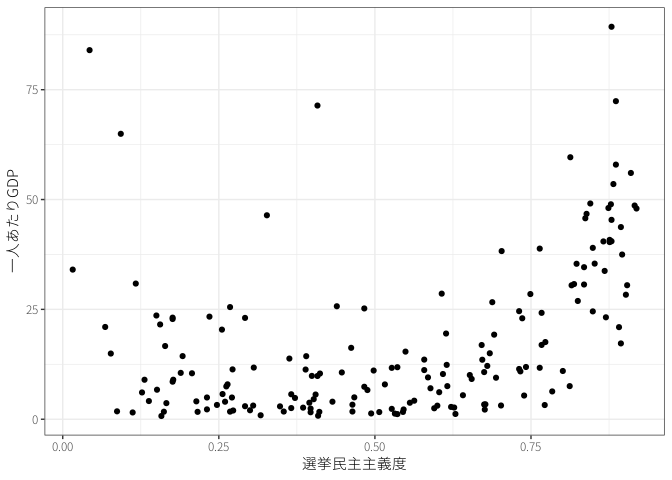
\includegraphics{liberal_peace_files/figure-pdf/unnamed-chunk-2-1.png}

}

\caption{安保理における拒否権の推移}

\end{figure}

唯一の例外として1950年の\textbf{朝鮮戦争}の際に\href{https://ja.wikisource.org/wiki/\%E5\%9B\%BD\%E9\%9A\%9B\%E9\%80\%A3\%E5\%90\%88\%E5\%AE\%89\%E5\%85\%A8\%E4\%BF\%9D\%E9\%9A\%9C\%E7\%90\%86\%E4\%BA\%8B\%E4\%BC\%9A\%E6\%B1\%BA\%E8\%AD\%B083}{安保理決議83}が採択され、国連軍が派遣された。\footnote{ソ連は中国の代表権を巡ってボイコットしており、拒否権を行使できなかった。}

\begin{itemize}
\tightlist
\item
  当時の韓国は国連加盟国ではなかったので、厳密な意味での集団安全保障ではない。
\item
  国連憲章上では国連軍の設立が予定されていたが(第43条)、現実的であるとは言えず、加盟国に武力行使を\textbf{授権}
  (authorize) する方針を取る。
\end{itemize}

\textbf{平和のための結集} (Uniting for Peace)
決議\(\leadsto\)拒否権が行使された場合に総会が勧告できるようにする。

\begin{tcolorbox}[enhanced jigsaw, rightrule=.15mm, breakable, bottomrule=.15mm, colback=white, left=2mm, toptitle=1mm, title=\textcolor{quarto-callout-note-color}{\faInfo}\hspace{0.5em}{平和のための結集決議 主文1}, colbacktitle=quarto-callout-note-color!10!white, titlerule=0mm, coltitle=black, bottomtitle=1mm, arc=.35mm, opacitybacktitle=0.6, leftrule=.75mm, colframe=quarto-callout-note-color-frame, toprule=.15mm, opacityback=0]

Resolves that if the Security Council, \textbf{because of lack of
unanimity of the permanent members}, fails to exercise its primary
responsibility for the maintenance of international peace and security
in any case where there appears to be a threat to the peace, breach of
the peace, or act of aggression, \textbf{the General Assembly} shall
consider the matter immediately with a view to making
\textbf{appropriate recommendations} to Members for collective measures,
including in the case of a breach of the peace or act of aggression
\textbf{the use of armed force} when necessary, to maintain or restore
international peace and security.

\end{tcolorbox}

\begin{itemize}
\tightlist
\item
  国連\href{https://www.un.org/en/ga/sessions/emergency.shtml}{緊急特別総会}
  (emergency special session: ESS) を開催
\item
  平和のための結集決議が最初に使われたのは1956年の\textbf{スエズ戦争}(第2次中東戦争)のときである。

  \begin{itemize}
  \tightlist
  \item
    イスラエルがエジプトのスエズ運河に侵攻し、利権を狙ったイギリスとフランスが介入
  \item
    アメリカとソ連が協力して緊急特別総会を招集し、第1次国連緊急軍 (UNEF
    I) を展開
  \item
    軽武装の軍隊を停戦地帯に派遣し、監視
  \end{itemize}
\end{itemize}

集団安全保障が想定する\textbf{平和執行} (peace-enforcement)
とは異なる\textbf{平和維持活動} (peacekeeping operation)\footnote{しばしば、日本語では平和維持活動をPKOと略すが、国際的には通用しない略称である。}
が発明

\begin{itemize}
\tightlist
\item
  最初の平和維持活動は第1次中東戦争の際の国連休戦監視機構
\item
  国連憲章には規定がないので「6章半\footnote{平和的解決の第6章と軍事制裁を含む強制措置の第7章の中間という意味。}の活動」と呼ばれる。
\item
  UNEF
  Iを主導したピアソンは1957年に、平和維持活動自体は1988年にノーベル平和賞を受賞
\end{itemize}

\begin{figure}[htpb]

{\centering 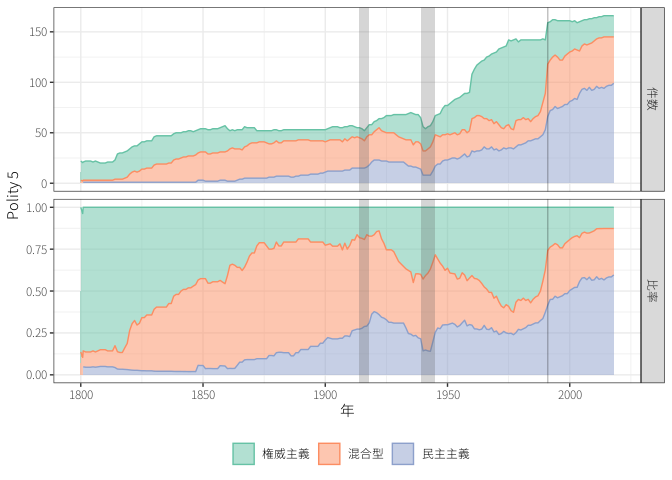
\includegraphics{liberal_peace_files/figure-pdf/unnamed-chunk-3-1.png}

}

\caption{平和維持活動の推移}

\end{figure}

\begin{figure}[htpb]

{\centering \includegraphics{liberal_peace_files/mediabag/1280px-UNpeacekeepin.png}

}

\caption{\href{https://commons.wikimedia.org/wiki/File:UNpeacekeeping.svg}{国連平和維持活動の展開}}

\end{figure}

\hypertarget{ux51b7ux6226ux5f8cux671fux5f85ux3068ux5931ux671b}{%
\subsection{冷戦後:期待と失望}\label{ux51b7ux6226ux5f8cux671fux5f85ux3068ux5931ux671b}}

冷戦の終結\(\leadsto\)イデオロギー対立が解消\(\leadsto\)安保理の活性化

\begin{figure}[htpb]

{\centering 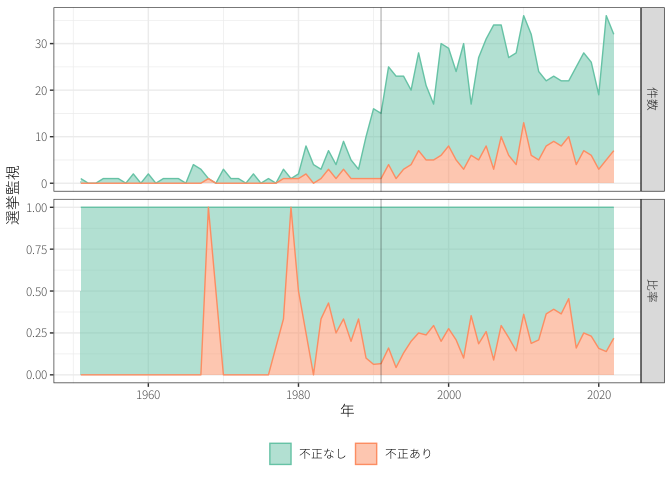
\includegraphics{liberal_peace_files/figure-pdf/unnamed-chunk-4-1.png}

}

\caption{安保理会合の推移}

\end{figure}

\begin{itemize}
\tightlist
\item
  代表的な例:1990年の\textbf{湾岸戦争}の際に\href{https://digitallibrary.un.org/record/102245}{安保理決議678}が採択され、国連軍が派遣
\item
  \href{https://research.un.org/en/docs/resolutions}{国連決議の読み方}
\end{itemize}

\begin{tcolorbox}[enhanced jigsaw, rightrule=.15mm, breakable, bottomrule=.15mm, colback=white, left=2mm, toptitle=1mm, title=\textcolor{quarto-callout-note-color}{\faInfo}\hspace{0.5em}{国連安保理決議678}, colbacktitle=quarto-callout-note-color!10!white, titlerule=0mm, coltitle=black, bottomtitle=1mm, arc=.35mm, opacitybacktitle=0.6, leftrule=.75mm, colframe=quarto-callout-note-color-frame, toprule=.15mm, opacityback=0]

\emph{The Security Council},

\emph{Recalling and reaffirming} its resolutions 660 (1990) of 2 August
1990, 661 (1990) of 6 August 1990, 662 (1990) of 9 August 1990, 664
(1990) of 18 August 1990, 665 (1990) of 25 August 1990, 666 (1990) of 13
September 1990, 667 (1990) of 16 September 1990, 669 (1990) of 24
September 1990, 670 (1990) of 25 September 1990, 674 (1990) of of 29
October 1990 and 677 (1990) of 28 November 1990.

\emph{Noting} that, despite all efforts by the United Nations, Iraq
refuses to comply with its obligation to implement resolution 660 (1990)
and the above-mentioned subsequent relevant resolutions, in flagrant
contempt of the Security Council,

\emph{Mindful of} \textbf{its duties and responsibilities} under the
Charter of the United Nations for \textbf{the maintenance and
preservation of international peace and security},

\emph{Determined} to secure full compliance with its decisions,

\emph{Acting} under \textbf{Chapter VII} of the Charter,

\begin{enumerate}
\def\labelenumi{\arabic{enumi}.}
\item
  \emph{Demands} that Iraq comply fully with resolution 660 (1990) and
  all subsequent relevant resolutions, and decides, while maintaining
  all its decisions, to allow Iraq one final opportunity, as a pause of
  goodwil, to do so;
\item
  \textbf{\emph{Authorizes}} Member States co-operating with the
  Government of Kuwait, unless Iraq on or before 15 January 1991 fully
  implements, as set forth in paragraph 1 above, the above-mentioned
  resolutions, to \textbf{use all necessary means} to uphold and
  implement resolution 660 (1990) and all subsequent relevant
  resolutions and to restore international peace and security in the
  area;
\item
  \emph{Requests} all States to provide appropriate support for the
  actions undertaken in pursuance of paragraph 2 of the present
  resolution;
\item
  \emph{Requests} the States concerned to keep the Security Council
  regularly informed on the progress of actions undertaken pursuant to
  paragraphs 2 and 3 of the present resolution;
\item
  \emph{Decides} to remain seized of the matter.
\end{enumerate}

\end{tcolorbox}

\begin{itemize}
\tightlist
\item
  国連決議の探し方:\href{https://rnavi.ndl.go.jp/jp/politics/UN-tool.html}{国会図書館}、\href{https://www.unic.or.jp/texts_audiovisual/libraries/research_guide/}{国連広報センター}

  \begin{itemize}
  \tightlist
  \item
    \href{https://research.un.org/en/docs/ga/quick/regular/76}{総会}、\href{https://www.un.org/securitycouncil/content/resolutions-0}{安保理}
  \end{itemize}
\item
  国連の文書記号:\href{https://rnavi.ndl.go.jp/jp/politics/UN-docOR.html}{国会図書館}、\href{https://www.unic.or.jp/texts_audiovisual/libraries/research_guide/research/symbols/}{国連広報センター}
\end{itemize}

武力行使授権(容認)決議の特徴:

\begin{enumerate}
\def\labelenumi{\arabic{enumi}.}
\tightlist
\item
  平和に対する脅威の認定
\item
  第7章(あるいは第42条)に基づく宣言
\item
  「すべての必要な措置を取る」ことの授権
\end{enumerate}

2001年の\textbf{9.11同時多発テロ}:加盟国に共通の脅威と認知\(\leadsto\)安保理決議1368

\begin{itemize}
\tightlist
\item
  テロリズムに対しても自衛権を行使
\item
  NATOは初めて集団的自衛権を行使\(\leadsto\)アフガニスタンへ侵攻
\end{itemize}

2003年の\textbf{イラク戦争}:はアメリカやイギリスが明確な武力行使授権決議なしに攻撃

\begin{itemize}
\tightlist
\item
  中国やロシアだけでなくフランスやドイツも反対
\end{itemize}

2014年のロシアによる\textbf{クリミア侵攻}、2022年の\textbf{ウクライナ侵攻}:安保理は機能不全

\(\leadsto\)安保理が対応できるのは、常任理事国間で利害が対立しない程度に重要ではなく、行動しようと思う程度には重要な事態である。


  \bibliography{references.bib}


\end{document}
